\chapter{Diseño de personajes}

% ==============================================================================

\section{Ingeniera \emph{(Nombre Provisional)}}

\subsection{Gameplay}
La ingeniera es un personaje que se especializa en el ataque a larga distancia mediante diversos tipos de proyectiles. Es un personaje que aporta una gran cantidad de daño y desde una distancia de seguridad a costa de tener poca vida y movilidad.

Para ser efectivo con ella, el jugador debe hacer todo lo posible por
alejarse cuanto más pueda de los enemigos y, entonces, atacarlos aprovechándose de su gran rango. Como la ingeniera solo tiene una habilidad para escapar del peligro, su $W$, sus habilidades requieren que se quede inmóvil para usarlas y tiene poca vida, esto hace que sus opciones de supervivencia sean muy limitadas si los enemigos consiguen cubrir la distancia que los separa. De esta forma, el gameplay de la ingeniera consiste en alejarse de los enemigos, atacarlos desde un lugar seguro y repetir este proceso cada vez que los enemigos consiguen acercarse.

\subsection{Habilidades}
\subsubsection{Habilidades básicas}
\begin{itemize}
\item \textbf{Ataque Básico.} Al hacer click en un enemigo le dispara con una ballesta. El disparo hace poco daño pero tiene bastante rango. Es la única habilidad que no necesita que se quede quieta para usarse.
\item \textbf{Q.} Saca una pistola y dispara un proyectil de alcance infinito pero que no atraviesa obstáculos.
\item \textbf{W.} Dispara un gancho de alcance medio que, al impactar con un obstáculo, lleva a la ingeniera hasta este. Para limitar sus opciones de movilidad, el CD de esta habilidad es elevado.
\item \textbf{E.} Dispara una granada. Esta granada es un proyectil lento que rebota con los obstáculos un número limitado de veces. Tras chocar con un enemigo o alcanzarse el número máximo de rebotes, la granada explota, infringiendo daño en un área pequeña. El número máximo de granadas que puede haber en un momento dado en el mapa es de 3.
\item \textbf{Ultimate (R).} Saca una pistola gigante que tiene un tiempo de carga de 4 segundos antes de poderse usar. Una vez que ha terminado el tiempo de carga, puede realizar 10 disparos en rápida sucesión que tienen alcance ilimitado y atraviesan todos los obstáculos y enemigos, causando daño moderado a los enemigos contra los que impactan. Durante todo el proceso que dure la habilidad, la ingeniera no puede moverse del sitio. Si recibe crowd control (CC) durante el tiempo de carga o de uso de la habilidad, la habilidad se cancela, con lo que puede volver a moverse. También puede elegir cancelar la habilidad en cualquier momento de carga o uso. Al cancelarse, la carga de la ulti vuelve a 0. Esta habilidad tiene un CD largo.
\end{itemize}

\subsection{Diseño}

\begin{figure}[h]
	\centering
	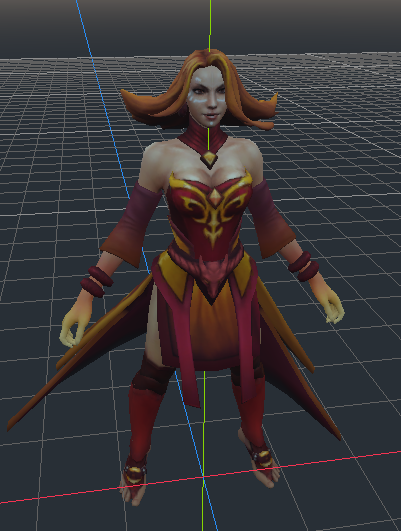
\includegraphics[width=0.6\linewidth]{figures/EngineerModel.png}
	\caption{Modelo Provisional de la Ingeniera.}
	\label{fig:EngineerModel}
\end{figure}

La ingeniera es una chica de complexión pequeña que lleva a la espalda una mochila, demasiado grande para ella, con todos los artilugios que usa para la batalla. El diseño del personaje está construido alrededor de este contraste, personaje pequeño con herramientas demasiado grandes para ella. Además, debido al gran peso de su mochila, se justifica que la ingeniera sea lenta y deba pararse siempre que usa una habilidad, debido al gran peso de las armas y a su difícil manejo. La ingeniera tiene también el pelo largo para enfatizar todavía más este contraste.

Este personaje estaría inspirado en el arquetipo ingeniero/artificiero de otros juegos. Como traje, llevaría un mono simple de trabajo y, aparte, unas gafas sobre la cabeza de estilo SteamPunk. El diseño de personaje debe transmitir que la ingeniera es un personaje muy inteligente que se ha valido de su gran inteligencia y habilidad para crear un gran conjunto de armas pero que, debido a su poca fuerza física y su torpeza, le cuesta usar sus propias creaciones.

En la figura \ref{fig:EngineerModel} se puede ver el modelo de la ingeniera que hemos usado como \emph{placeholder} (modelo provisional) para este proyecto. Este modelo es el del personaje \emph{Lina} del videojuego Dota 2, que se ha descargado de la siguiente página: \emph{http://www.dota2.com/workshop/requirements}.

\subsection{Sonido}
Los efectos de sonido de las habilidades de la Ingeniera están asociados a disparos, tanto de pistolas como de arcos y otras armas. Aparte, su ultimate tiene un sonido de carga, que se reproduce durante los 4 segundos que dura el casteo.

% --------------------------------------------------------------

\section{Bardo \emph{(Nombre Provisional)}}

\subsection{Gameplay}
El bardo es un flautista support caracterizado por aplicar buffos en areas de efecto alrededor suya. Apenas aporta daño al equipo pero aumenta las capacidades de supervivencia de este.

El bardo cuenta con un sistema de recursos: Melodías. Cada habilidad básica genera una melodía que se va almacenando hasta un máximo de 3. Estas melodías se pierden cuando el bardo sufre una cierta cantidad de daño o CC. Una vez se alcanza el máximo de melodías, la producción de otra elimina la primera de ellas.
Las melodías mejoran los stats de la habilidad que la producen y aplica un efecto temporal en el ataque básico (esto último es importante porque sino un healer y un tanque no tienen mucha viabilidad y están condenados desde el primer momento), y pueden ser descargados en la R para generar un gran área de efecto con efectos especiales. Los stats también se acumulan según el número de melodías.

La forma de jugar del bardo es cerca de su aliado, protegiendo y eligiendo cuidadosamente la melodías que desea mantener. Puesto que los efecctos de la R dependen de las últimas 3 melodías, y que el casting de estas lleva su tiempo, debe tener buena visión de futuro sobre la situación del juego a la que se va a enfrentar.

\subsection{Habilidades}
\subsubsection{Habilidades básicas}
Q-W-E tienen un cooldown medio (ej: 5s) y mientras se utilizan el bardo no puede atacar (pero sí moverse). Durante la duración de la habilidad se aplica el efecto, una vez acaba desaparece (excepto los stats de las melodías). La R tiene un cooldown bajo para una habilidad final (ej: 20 s), y se aplica inmediatamente tras un pequeño casting.

\begin{itemize}
    \item \textbf{Ataque Básico.} Dispara un dardo con la flauta. Mantiene un rango relativamente alto pero con muy poco daño. Poca velocidad de disparo.
    \item \textbf{Q.} Cura durante unos segundos alrededor suya. Sus básicos adquieren robo de vida.
    \item \textbf{W.} Aumenta la velocidad de ataque y de movimiento de los aliados en el área.
    \item \textbf{E.} Aumenta el daño básico de los aliados en el área.
    \item \textbf{Ultimate (R).} Descarga las melodías almacenadas en un gran área de efecto alrededor suya. Si el bardo no tiene 3 melodías en ese momento únicamente se juntan los efectos de las que haya, en caso de que haya 3:
    \begin{itemize}
        \item Q-Q-Q: Cura al máximo y revive a los aliados en el área. (El revivir puede estar demasiado roto, quizás transformarlo por: aumentar la vida máxima de los personajes temporalmente)
        \item W-W-W: Aumenta en gran medida la velocidad de ataque y de movimiento y de aliados. Durante ese tiempo pueden atravesar unidades (quizás no es muy fuerte)
        \item E-E-E: Los enemigos reciben más daño durante los siguientes segundos.
        \item Q-W-E: Stunea a todos los enemigos de la zona durante unos segundos.
        \item Q-Q-W: Por decidir.
        \item Q-Q-E: Por decidir.
        \item W-W-Q: Por decidir.
        \item W-W-E: Por decidir.
        \item E-E-Q: Por decidir.
        \item E-E-W: Por decidir.
    \end{itemize}
\end{itemize}

\subsection{Diseño}
Podría orientarse como un flautista de Hamelín con un toque más misterioso. Podría llevar capa y una bolsa de la que sobresalen partituras. Puesto que dispara dardos, podrían salirle de un compartimento que tenga en el brazo.

Las áreas de efecto de las habilidades deberían diferenciarse con claridad (podrían estar acompañadas con dibujos de notas musicales, aunque quizás sobrecargue demasiado). Sería recomendable que cada una se asociase con un color primario diferente (pero con cuidado con no saturarse con el terreno). Las ultis podrían separar el área en diferentes colores según las habilidades o podrían consistir de la combinación de sus colores.

\subsection{Sonido}
Cada habilidad debería producir una melodía diferente (preferiblemente de flauta). De la misma manera cada versión de la R vendría acompañada de un sonido diferente (preferiblemente con orquestación)

% --------------------------------------------------------------

\section{Mago \emph{(Nombre Provisional)}}

\subsection{Gameplay}
El mago es un personaje de apoyo que se especializa en el control del mapa, proporcionando protección a su aliado y evitando que los enemigos puedan llegar hasta él. Al contrario que en otros juegos, es bastante \emph{tanque}, lo que le permite preocuparse menos por su seguridad centrándose casi por completo en mantener a su aliado vivo y en darle apoyo.

Sus habilidades giran entorno al control del mapa y al posicionamiento de los distintos jugadores: él, su aliado y el equipo enemigo. Debe mantener alejado a su aliado del equipo enemigo, de ahí que tenga especial sinergia con campeones frágiles y/o con poca movilidad que tienen ataques a larga distancia. Su posicionamiento, en cambio, debe ser totalmente opuesto. Debido a sus habilidades y a su gran aguante, debe intentar siempre ``estar en medio'' del equipo enemigo, molestándolos e impidiéndoles llegar hasta su aliado.

\subsection{Habilidades}
\subsubsection{Habilidades básicas}
\begin{itemize}
\item \textbf{Ataque Básico.} Al hacer click en un enemigo le da un golpe con su bastón. Este ataque, de corto alcance, hace muy poco daño pero invoca al hielo para aplicar una ralentización pequeña durante un periodo de tiempo medio.
\item \textbf{Q.} Invoca un elemento al azar sobre una zona. Los enemigos que pasen sobre esa zona recibirán un debuff que dependerá del tipo de elemento. De la misma forma, los proyectiles aliados que pasen sobre esa zona aplicarán el mismo debuff al impactar. Los elementos y sus debuffs asociados son: hielo - ralentización, fuego - daño por segundo, veneno - vulnerabilidad (aumenta el daño recibido por los siguientes ataques). Para usar esta habilidad, el jugador debe poner el ratón en la zona donde quiere castearla y pulsar la tecla \emph{Q}.
\item \textbf{W.} Intercambia su posición por la de su aliado.
\item \textbf{E.} Levanta un muro de piedra en la posición deseada. El funcionamiento es el siguiente: el jugador debe pulsar la tecla \emph{E} en un punto y después volver a pulsarla con el ratón en otro punto, para crear un muro que vaya de un punto al otro. Si ambos puntos están demasiado lejos entre sí, el muro será desde el primer punto hacia el segundo punto pero se \emph{cortará} antes de llegar a este último. De la misma forma, si ambos puntos están demasiado cerca, no se construirá el muro porque sería demasido pequeño. El muro permanece en el mapa hasta que el jugador construye otro.
\item \textbf{Ultimate (R).} Tras un largo tiempo de casteo (que no puede cancelar y durante el cual no puede ejecutar ninguna acción ni moverse) invoca a una tormenta que \emph{stunea} a los enemigos en una zona alrededor suya. Estos enemigos no podrán moverse ni realizar ninguna otra acción durante 5 segundos (tiempo de duración del \emph{stun}).
\end{itemize}

\subsection{Diseño}

\begin{figure}[h]
	\centering
	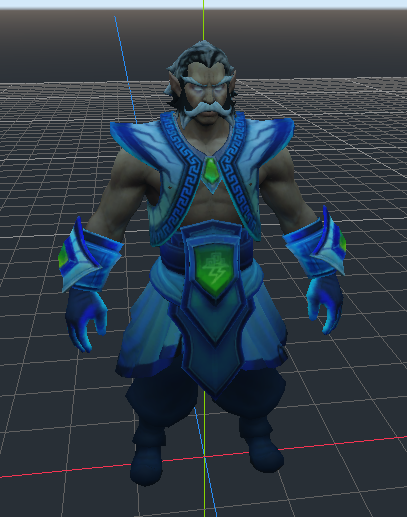
\includegraphics[width=0.6\linewidth]{figures/MageModel.png}
	\caption{Modelo Provisional del Mago.}
	\label{fig:MageModel}
\end{figure}

El mago es un hombre de complexión fuerte que está ataviado con una túnica y un gran bastón mágico, que usa para todos sus ataques. Al igual que la ingeniera, este personaje también se basa en un contraste: fuerza vs inteligencia, físico vs mental. Por una parte, este personaje es fuerte. Su misión es \emph{tanquear} al equipo enemigo mientras protege a su aliado. Por otra parte, al ser un mago, todas sus habilidades (menos su ataque básico) giran alrededor de su magia. Su diseño debe reflejar este contraste, manteniendo a la vez un equilibrio entre ambas facetas.

Todas sus habilidades usan/invocan algún elemento. Su ataque básico usa hielo. Su \emph{Q} usa hielo, fuego o veneno, según el efecto escogido al azar. Su \emph{W} usa aire (teletransportación). Su \emph{E} usa tierra (invoca un muro de roca). Su \emph{R} usa rayo (invoca una tormenta).

En la figura \ref{fig:MageModel} se puede ver el modelo del mago que hemos usado como \emph{placeholder} para este proyecto. Este modelo es el del personaje \emph{Zeus} del videojuego Dota 2, que se ha descargado de la siguiente página: \emph{http://www.dota2.com/workshop/requirements}.

\subsection{Sonido}
Los efectos de sonido de las habilidades del Mago están asociados a magia y elementos (como el sonido de tormenta que se reproduce cuando activa su ultimate). Además, mientras castea su ultimate, se reproduce un efecto de sonido que avisa a los enemigos de que se tienen que alejar del Mago para no ser stuneados.